\documentclass[11pt,a4paper]{article}
\usepackage[margin=2.2cm]{geometry}
\usepackage{amsmath,amssymb}
\usepackage{graphicx}
\usepackage{booktabs}
\usepackage{listings}
\usepackage{xcolor}
\usepackage[hidelinks]{hyperref}

\lstset{basicstyle=\ttfamily\small, keywordstyle=\color{blue!70!black}, commentstyle=\color{gray},
        language=Python, frame=single, columns=fullflexible, showstringspaces=false}

\title{CSE485/CSE488 Deep Learning\\[2pt] \large Assignment 1: MicroGrad (Scalar Autograd Engine)}
\author{Abdelmoneim Mahmoud \quad (23P0015)\\[2pt]
\small Branch: \texttt{abdelmoneim-mahmoud\_23P0015} \quad PR: \url{https://github.com/DL-Course-ASU/assignment-1-micrograd-template/pull/1}}
\date{}

\begin{document}
\maketitle

\section{Overview}
\texttt{src/engine.py} implements a \texttt{Value} class. It wraps one scalar, records the operation that produced it, and stores a gradient.
\texttt{src/nn.py} builds \texttt{Neuron}, \texttt{Layer} and \texttt{MLP} on top of it.
All 12 tests in the template pass (\texttt{python -m pytest}), and \texttt{demo.ipynb} trains an MLP on the two-moons dataset.

\section{Mathematical Derivations}
Each operation creates an output node $o=f(a,b)$. During backpropagation the node already holds
$\frac{\partial L}{\partial o}$ (\texttt{out.grad}). The chain rule then gives the contribution to each input:
\[
  \frac{\partial L}{\partial a} \mathrel{+}= \frac{\partial o}{\partial a}\cdot\frac{\partial L}{\partial o}.
\]
Each \texttt{\_backward} closure only needs the \emph{local} derivative $\partial o/\partial a$:

\begin{center}
\begin{tabular}{@{}lll@{}}
\toprule
Operation & Forward & Local derivative(s) \\
\midrule
Addition & $o=a+b$ & $\partial o/\partial a = 1,\ \partial o/\partial b = 1$ \\
Multiplication & $o=a\,b$ & $\partial o/\partial a = b,\ \partial o/\partial b = a$ \\
Power ($n$ constant) & $o=a^{n}$ & $\partial o/\partial a = n\,a^{\,n-1}$ \\
Exponential & $o=e^{a}$ & $\partial o/\partial a = e^{a} = o$ \\
Tanh & $o=\tanh a$ & $\partial o/\partial a = 1-\tanh^2 a = 1-o^2$ \\
\bottomrule
\end{tabular}
\end{center}

\paragraph{Tanh.} $\tanh a = \frac{e^{a}-e^{-a}}{e^{a}+e^{-a}}$. The quotient rule gives
$\frac{d}{da}\tanh a = \frac{(e^{a}+e^{-a})^2-(e^{a}-e^{-a})^2}{(e^{a}+e^{-a})^2} = 1-\tanh^2 a$.
This is why the closure can reuse the forward output $t$ and skip any extra exponentials.

\paragraph{Derived operations.} These are built from the primitives above, so they need no backward code of their own:
\[
  -a = a\cdot(-1),\qquad a-b = a+(-b),\qquad a/b = a\cdot b^{-1}.
\]
For division, the power rule gives $\frac{\partial}{\partial b}\,a\,b^{-1} = -a\,b^{-2}$ automatically.
If $b=0$, computing $b^{-1}$ raises \texttt{ZeroDivisionError} in the forward pass, which is what the tests expect.

\paragraph{Why \texttt{+=}.} If a node feeds into several parents, the multivariable chain rule says
$\frac{\partial L}{\partial a}=\sum_{k}\frac{\partial L}{\partial o_k}\frac{\partial o_k}{\partial a}$.
Each parent adds its own term, so the gradient must be accumulated (\texttt{+=}) and not overwritten.
Example: for $d=(a+a)\,a=2a^2$ we need $\partial d/\partial a=4a=12$ at $a=3$.

\section{Topological Sort and \texttt{backward()}}
\begin{lstlisting}
def _get_topo(self):
    topo, visited = [], set()
    def build_topo(node):
        if node not in visited:
            visited.add(node)
            for child in node._prev:
                build_topo(child)
            topo.append(node)        # post-order
    build_topo(self)
    return topo

def backward(self):
    topo = self._get_topo()
    self.grad = 1.0                  # dL/dL = 1
    for node in reversed(topo):
        node._backward()
\end{lstlisting}

\paragraph{Post-order.} A node is appended only \emph{after} all of its inputs. So in \texttt{topo} every node comes after the nodes it depends on.
Reversing the list puts every node \emph{before} its inputs.
When a node's \texttt{\_backward} runs, every parent that uses it has already finished, and its \texttt{grad} is complete.
If we appended before visiting the children, a node could push its gradient down before receiving all of its own.

\paragraph{Visited set (diamond graph).} Take $c=a+a$. The node $a$ appears twice in the graph but must appear
\emph{once} in \texttt{topo}, otherwise its \texttt{\_backward} would run twice and double-count.
Trace: \texttt{build\_topo(c)} visits $a$ and appends it, so \texttt{topo}$=[a, c]$.
Then $c$.\texttt{grad}$=1$, and $c$.\texttt{\_backward} adds $1$ to $a$.\texttt{grad} once for each operand (\texttt{self} and \texttt{other} are both $a$), giving
$a.\texttt{grad}=2=\frac{d(2a)}{da}$. Without the set, large graphs with shared nodes would also be revisited an exponential number of times.
The set hashes nodes by identity. That is why \texttt{Value} does not override \texttt{\_\_eq\_\_}: two nodes with equal data must not collapse into one.

\section{Design Justifications}
\begin{itemize}
  \item \textbf{Strict input types.} \texttt{\_\_add\_\_} and \texttt{\_\_mul\_\_} wrap only \texttt{int}/\texttt{float}/\texttt{Value} and raise \texttt{TypeError} otherwise
        (for example \texttt{Value(2) + "string"}). Strings and lists would otherwise produce silent nonsense.
  \item \textbf{Power with a constant exponent only.} \texttt{\_\_pow\_\_} asserts the exponent is \texttt{int}/\texttt{float}, as the template and tests require.
        A \texttt{Value} exponent would need $\partial(a^b)/\partial b = a^b\ln a$, which is undefined for $a\le 0$.
  \item \textbf{Reverse operators.} \texttt{\_\_radd\_\_}, \texttt{\_\_rmul\_\_}, \texttt{\_\_rsub\_\_} and \texttt{\_\_rtruediv\_\_} make \texttt{2 + a}, \texttt{1 - a} and \texttt{2 / a} work.
        \texttt{\_\_radd\_\_} also lets Python's \texttt{sum()} start from \texttt{0}.
  \item \textbf{Closures for \texttt{\_backward}.} Each closure captures its own \texttt{self}, \texttt{other} and \texttt{out}, so the graph needs no separate operation table.
  \item \textbf{Neural-network API.} \texttt{Neuron} computes $\tanh(\mathbf{w}\cdot\mathbf{x}+b)$ with $w_i,b\sim U(-1,1)$.
        \texttt{Layer} returns a single \texttt{Value} when it has one neuron (this makes scalar losses easy).
        \texttt{parameters()} flattens recursively, and \texttt{zero\_grad()} calls \texttt{reset\_grad()} on every parameter.
  \item \textbf{Linear output layer.} \texttt{Neuron} has an optional \texttt{nonlin} flag (default \texttt{True}, so the tests behave exactly as specified).
        \texttt{MLP} turns it off for the last layer only. A tanh output is bounded in $[-1,1]$, so the hinge loss $\max(0,1-y\,s)$ could never be fully satisfied and its gradient would shrink near saturation.
        A linear output gives an unbounded score $s$ and avoids this. The same design is used in Karpathy's micrograd and in standard classifiers (logits).
\end{itemize}

\section{Conceptual Questions}
\paragraph{Q1. Why reverse-mode differentiation for neural networks?}
Training has one scalar output (the loss) and many inputs (the parameters). Reverse mode computes \emph{all}
$\partial L/\partial \theta_i$ in one backward pass, costing about as much as the forward pass.
Forward mode would need one pass per parameter (337 passes for our MLP, millions for real networks).

\paragraph{Q2. Why must \texttt{+=} be paired with \texttt{zero\_grad()}?}
Accumulation is correct \emph{within} one backward pass (shared nodes, Section 2).
Across training steps, though, \texttt{grad} would keep the previous step's values, and the update would use a stale running sum.
So \texttt{zero\_grad()} is called before every \texttt{backward()}. Fresh intermediate nodes are rebuilt every forward pass, so only the parameters need resetting.

\paragraph{Q3. What happens to gradients when tanh saturates?}
$\tanh'(a)=1-\tanh^2 a\to 0$ as $|a|$ grows. In a deep stack these factors multiply,
so gradients for early layers can vanish. Mitigations: small initial weights, normalised inputs, ReLU-type activations, normalisation layers.

\paragraph{Q4. What is the cost of a scalar engine compared with PyTorch?}
Every scalar operation is a Python object plus a closure. Our 100-sample, 337-parameter MLP builds a graph of about 69{,}000 nodes per step, and the notebook takes about 1--2 minutes for 100 steps.
PyTorch represents a whole matrix multiply as \emph{one} node with a tensor-level backward ($\partial L/\partial W = \delta\,x^\top$) running in optimised C++/CUDA.
The maths is identical. Only the granularity of the nodes changes.

\paragraph{Q5. Why do we need the recursion limit in the demo?}
\texttt{\_get\_topo} is recursive, and its depth equals the longest path in the graph.
Summing 100 losses and 337 squared parameters with \texttt{sum()} creates a chain several hundred nodes long, close to Python's default limit of 1000.
The notebook raises the limit with \texttt{sys.setrecursionlimit}. An iterative DFS would avoid it, but the recursive version follows the assignment's hint directly.

\section{Demo Results (\texttt{demo.ipynb})}
\begin{itemize}
  \item \textbf{Gradient check.} For $f(a,b)=\tanh\!\big(\tfrac{ab+b^3}{a-4}\big)+e^{a/2}-2/b$, every operator is used.
        The autograd gradients match central finite differences ($h=10^{-6}$) to 6 decimal places:
        $\partial f/\partial a = 1.432677$, $\partial f/\partial b = 3.197680$.
  \item \textbf{Training.} \texttt{make\_moons} (100 points, noise 0.1), \texttt{MLP(2,[16,16,1])} with 337 parameters,
        mean hinge loss with $10^{-4}$ L2, and SGD with the learning rate decaying from 1.0 to 0.1 over 100 steps.
        Loss drops from 0.866 to 0.014, and training accuracy reaches 100\% by step 30.
\end{itemize}

\begin{figure}[h]
  \centering
  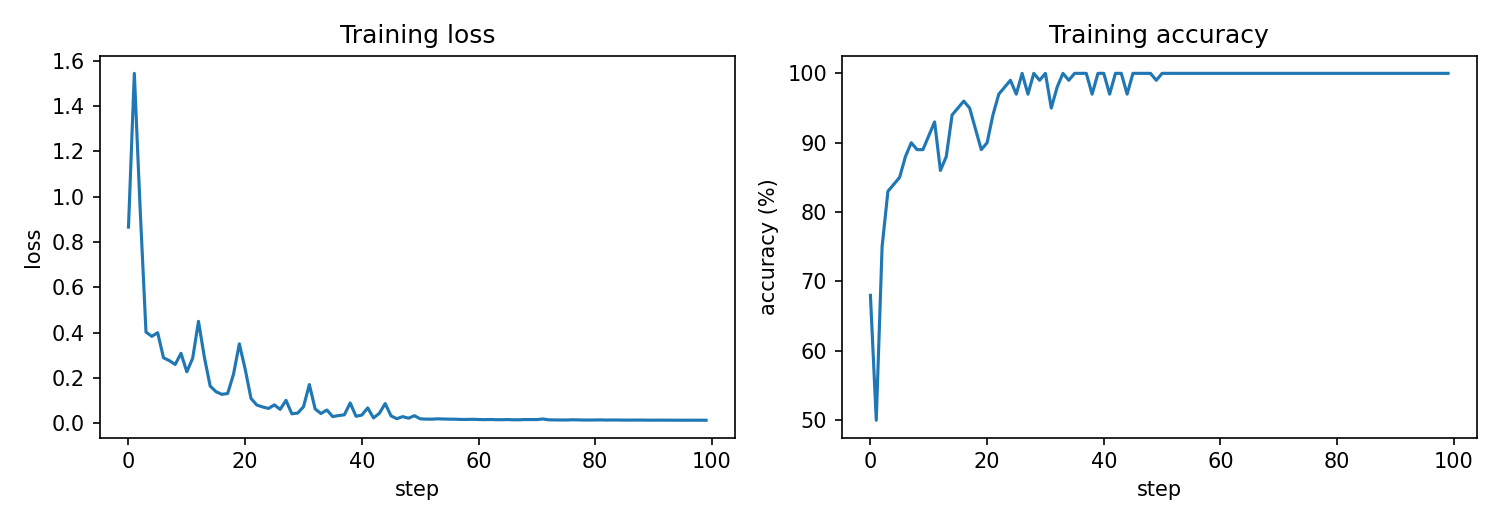
\includegraphics[width=0.95\linewidth]{figures/curves.png}
  \caption{Training loss and accuracy.}
\end{figure}
\begin{figure}[h]
  \centering
  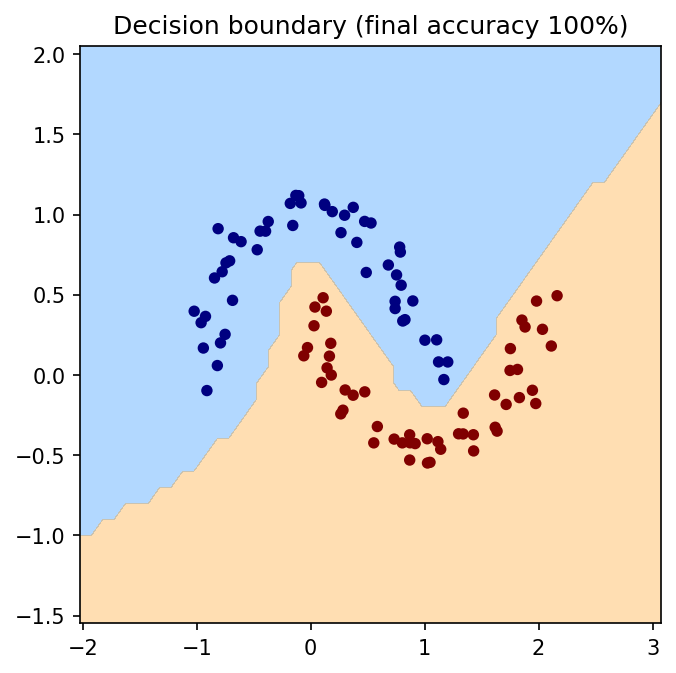
\includegraphics[width=0.48\linewidth]{figures/boundary.png}
  \caption{Learned decision boundary on the two-moons data.}
\end{figure}

\end{document}
